\chapter{Lösungsansatz}
\label{ch:solution}
Bei den Dokumenten handelt es sich um stenografische Berichte des deutschen Bundestages, weswegen angenommen wurde das alle Dokumente eine Konsistenz in der Formatierung des Textblockes besitzen. Somit befasste sich das Teilprojekt \textit{Textextraktion-18} vorerst mit der Extraktion eines Dokumentes, beispielhaft sollte dies das XML-Dokument 18003.xml sein.
\section{Analyse der XML-Dokumente}
\subsection{Inhaltsverzeichnis}
\label{subsec:toc}
Bereits nach kurzer Analyse des Dokuments stellte sich eine Auffälligkeit innerhalb des Inhaltsverzeichnisses heraus. Alle Kapitel wurden mit ihrem Titel, dem dazugehörigem Abschnitt im Protokoll und den beteiligten Sprechern gelistet (siehe \autoref{img:toc}).
\begin{figure}[h]
	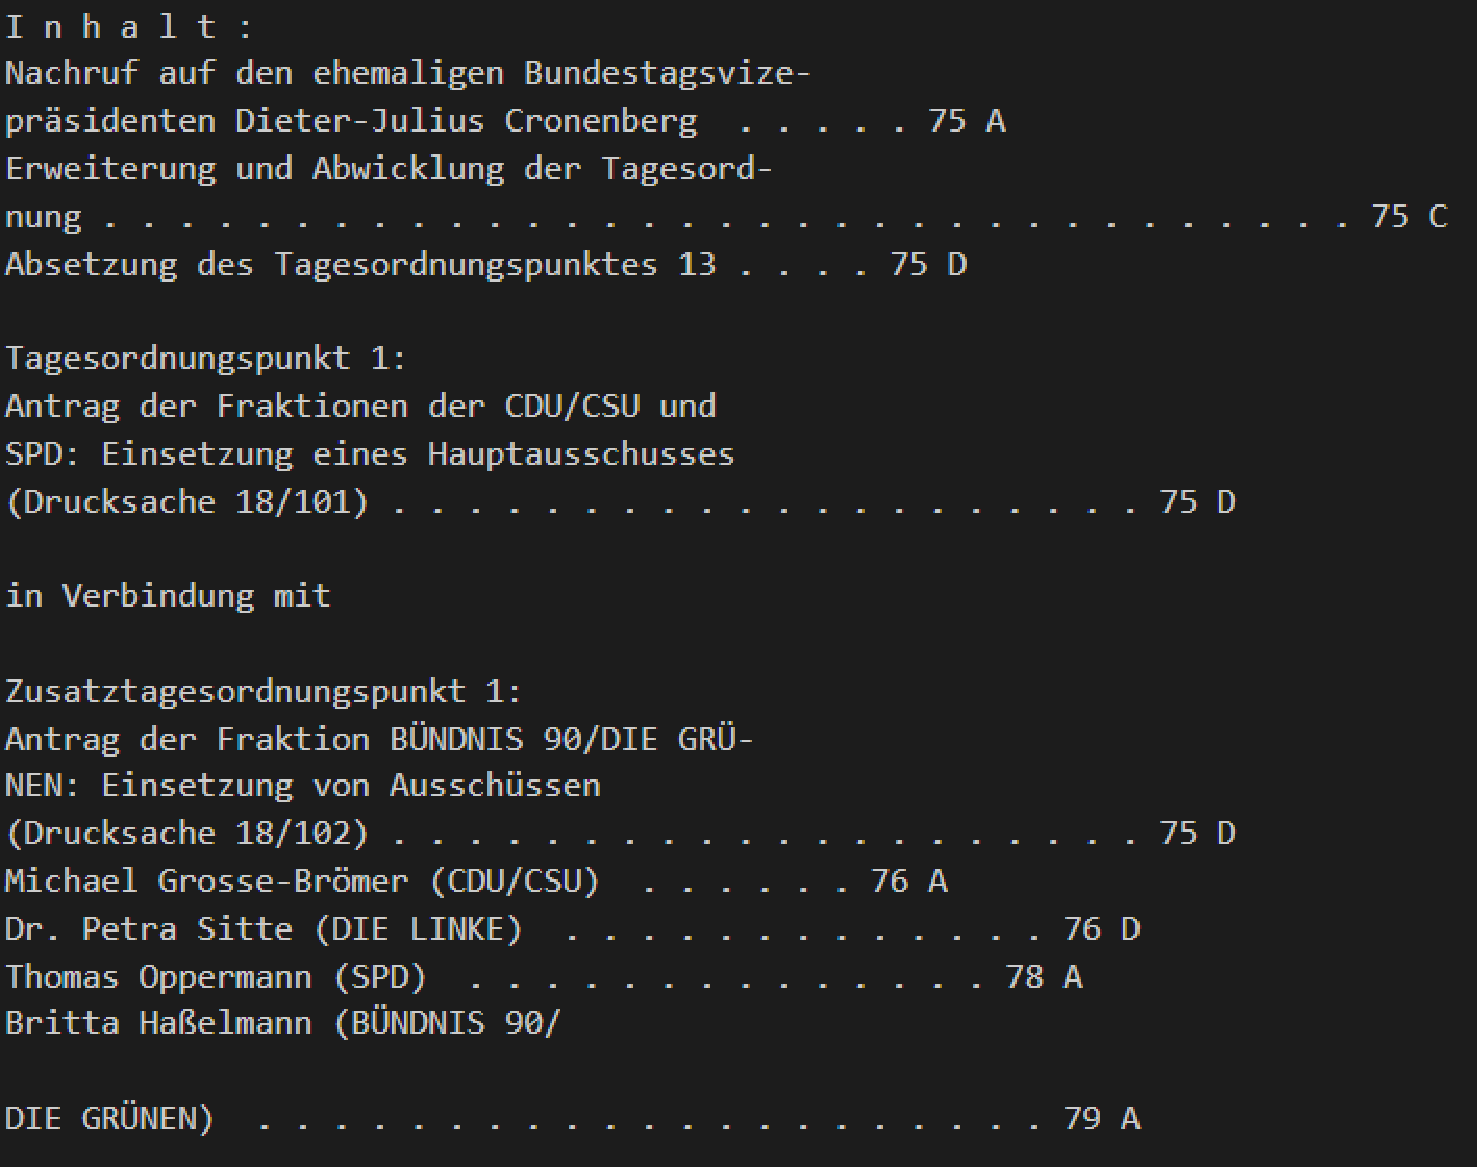
\includegraphics[width=\linewidth]{img/toc.pdf}
	\caption{Ansicht des Inhaltsverzeichnisses}
	\label{img:toc}
\end{figure}\newpage \noindent
\subsection{Eröffnungsrede}
\label{subsec:openning}
Zusätzlich wurde bei kurzem Vergleich mit wenigen anderen Dokumenten festgestellt, dass die Eröffnungsrede des Alterspräsident(siehe \autoref{img:begin}) scheinbar immer gleich eingeleitet wurde: \gequote{Beginn: 10.00 Uhr} (natürlich mit abweichender Uhrzeit)
\begin{figure}[h]
	\centering
	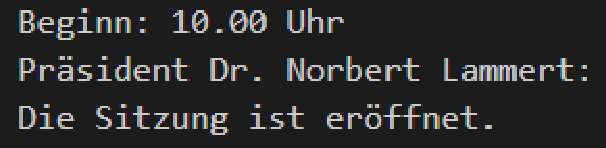
\includegraphics[width=.7\linewidth]{img/begin.pdf}
	\caption{Einleitung der Eröffnungsrede}
	\label{img:begin}
\end{figure}
\subsection{Redner}
\label{subsec:speech}
Darüber hinaus beginnt jede Rede mit dem Namen des Sprechenden und dessen Zugehörigkeit
\begin{figure}[h]
	\begin{minipage}{.42\linewidth}
		
\includegraphics[width=\linewidth]{img/petra.pdf}
	\end{minipage}\hfill
	\begin{minipage}{.54\linewidth}
		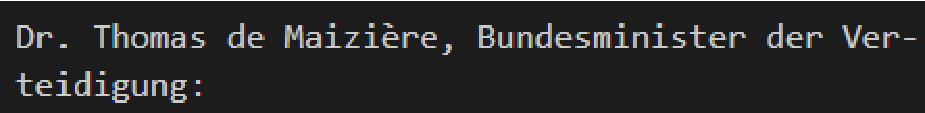
\includegraphics[width=\linewidth]{img/thomas.pdf}
	\end{minipage}
\end{figure}

\section{Extraktion mit Regulären Ausdrücken}
Es entwickelte sich die Idee anhand der Analyse reguläre Ausdrücke zu entwickeln die innerhalb des Textblockes passten (matchen). Für die einzelnen Teile der Analyse wurde dies wie folgt realisiert:
\begin{table}[h]
	\begin{tabularx}{\linewidth}{l X}
		\textbf{Analyseteil} & \textbf{regulärer Ausdruck in der Aufzählungsklasse}\\
		Inhaltsverzeichnis & \lstinline|TOC_NAMES(Pattern.compile("\\d\\s[A-Z]\\n+"))|\\
		Eröffnungsrede & \lstinline|OPENING(Pattern.compile("(Uhr(\\r\|\\n\|(\\n)*)(?=(Vize\|Alters)?(P\|p)räsident(en\|in\|innen)?))"))|\\
		Redner & \lstinline|BREAKINGPOINT(Pattern.compile("(.+,\\s.+minister.+\\r*\\n*.+:\\n)\|((.+p\|P)räsident.+:\\n)\|(.+\\(.+\\):\\n)\|(.+\\(.+/.+-\\r*\\n*.+\\):\\n)\|(.+\\(.+\\r*\\n*.+\\):\\n)\|(.+,.+kanzler.+:\\n)"))|\\
	\end{tabularx}
\end{table}

\newpage
\section{Theoretischer Ablauf}
Das zu erstellende Programm sollte nun grob wie folgt ablaufen:
\begin{enumerate}
	\item Einlesen des Dokuments, einzig relevante XML Tags sind \lstinline|<DATUM>| und \lstinline|<TEXT>|
	\item Alle Suchalgorithmen laufen innerhalb des Textblockes ab, das heißt im \lstinline|<TEXT>| Tag
	\item Durchsuche jeden Eintrag im Inhaltsverzeichnis nach Titeln und den dazugehörigen Rednern.
	\item Das Ende des Inhaltsverzeichnisses ist der Beginn der Eröffnungsrede des Alterspräsidenten.
	\item Alle nachträglichen Reden sollen dem Titel aus dem Inhaltsverzeichnis zugeordnet werden.
	\item Das Ende jeder Rede ist der Beginn einer neuen und kann mit dem \lstinline|BREAKINGPOINT| gefunden werden.
	\item Wurden alle Reden des Dokumentes gefunden sollen sie als JSON Datei gespeichert werden.
\end{enumerate}

\noindent im GitHub erreichbar unter:\\ \url{https://github.com/htw-projekt-p2p-volltextsuche/textextraction-18}